\documentclass{beamer}


\usetheme[progressbar=frametitle]{metropolis}
\usepackage{appendixnumberbeamer}

\usepackage{booktabs}
\usepackage[scale=2]{ccicons}
\usepackage{textpos}
\usepackage{xcolor,colortbl}
\usepackage{pgfplots}
\usepgfplotslibrary{dateplot}
\usepackage{url}
\usepackage[utf8]{inputenc}
\usepackage[T1]{fontenc}
\usepackage{tikzstyles}
\usepackage{textcomp}
\usepackage{pgfplots}
\usepackage{ulem}
\pgfplotsset{compat=1.14}
\usepackage{subfigure} 
\usepackage{mathabx}

\usepackage[
	backend=biber,
	citestyle=authoryear,
	bibstyle=authoryear,
	maxnames=2]{biblatex}
	\bibliography{bibliography.bib}

\usepackage{caption}
\captionsetup{font=scriptsize,labelfont=scriptsize}

% Math symbols
\newcommand{\E}{\mathbb{E}}
\newcommand{\Var}{\mathrm{Var}}
\newcommand{\Cov}{\mathrm{Cov}}

\newcommand\independent{\protect\mathpalette{\protect\independenT}{\perp}}
\def\independenT#1#2{\mathrel{\rlap{$#1#2$}\mkern2mu{#1#2}}}
\DeclareMathOperator*{\argmax}{arg\,max}

\tikzset{
  block/.style    = {draw, thick, rectangle, minimum height = 3em, minimum width = 3em},
  causalvar/.style      = {draw, circle, node distance = 2cm}
}

% Criteo colors/template (legacy)
\definecolor{criteoOrange}{RGB}{248,152,29}

% New names
\definecolor{cOrange}{RGB}{248,152,29}
\definecolor{cBlue}{RGB}{43,46,173}
\definecolor{cGreen}{RGB}{20,171,103}
\definecolor{cRed}{RGB}{248,88,29}

\setbeamercolor{structure}{fg=cOrange,bg=white}
\usepackage{helvet}
\setbeamertemplate{blocks}[rounded]

% https://www.overleaf.com/latex/templates/metropolis-beamer-theme/qzyvdhrntfmr
\addtobeamertemplate{frametitle}{}{%
\textblockcolour{white}
\begin{textblock*}{100mm}(.825\textwidth,-1.08cm)%.825\textwidth,,-1cm)

\includegraphics[scale=.205]{CAIL_logo}%0.3
\end{textblock*}}

\setbeamerfont{normal text}{size=\small}

\title{Generative Networks}

\author{Thomas Ricatte}

\date{2018-02-15}

\begin{document}

\begin{frame} 	 
\titlepage
\end{frame}

\begin{frame}[fragile]{Outline}
  \tableofcontents
\end{frame}

\section{Motivation}

\begin{frame}{Generative Networks}

\begin{itemize}
    \item A \emph{discriminative} model is a way to model the conditional probability of a target \textcolor{cOrange}{$Y$ (low-dimension)} given some covariates \textcolor{cBlue}{$X$ (high-dimension)}.
    \item Conversely, a \emph{generative} model tries to model the conditional probability of \textcolor{cBlue}{$X$} given \textcolor{cOrange}{$Y$} (or even the joint probability $\textcolor{cBlue}{X} \times \textcolor{cOrange}{Y}$
\end{itemize}
\begin{figure}
    \centering
    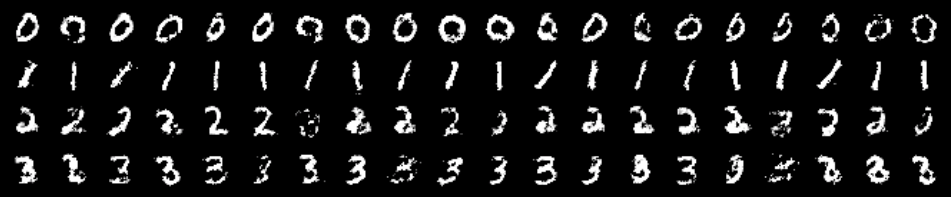
\includegraphics[width=0.7\linewidth]{images/conditional_mnist.png}
    \caption{Sampling from $P(X|Y)$ on MNIST using a ConditionalGan (\cite{cgan})}
\end{figure}
\end{frame}

\begin{frame}{Inverse convolutions}
    \begin{itemize}
    \item Our objective is to expand the signal from a \textcolor{cOrange}{low-dimension} representation to an \textcolor{cBlue}{high-dimension} signal space.
    \item In feed-forward networks, the objective was to reduce the signal dimension using for instance conv layers
    \end{itemize}
    \begin{figure}
        \centering
        \begin{tikzpicture}
        \draw[fill=cGreen!20] (0,0) -- (0,1) -- (1, 0.75) -- (1, 0.25) -- (0,0);
        \draw[bigarrow] (1.5, 0.5) -- (2.5, 0.5);
        \draw[fill=cGreen!20] (3,0.25) -- (3,0.75) -- (4, 1) -- (4, 0) -- (3,0.25);
        \end{tikzpicture}
    \end{figure}
    \begin{itemize}
        \item To do the opposite, we introduce the \emph{inverse convolutional} operator
    \end{itemize}
\end{frame}

\begin{frame}{Inverse convolutions (1D case)}

\begin{figure}
    \begin{tikzpicture}
    \draw (0.8, 0) node[tablecell]{1};
    \draw (1.6, 0) node[tablecell]{4};
    \draw (2.4, 0) node[tablecell]{-1};
    \draw (3.2, 0) node[tablecell]{0};
    \draw (4, 0) node[tablecell]{2};
    
    \draw[->,double,color=cBlue!15] (2.4, -0.4) -- (2.4, -1.6);
    
    \draw (0.8, -1) node{Conv};
    \draw (2, -1) node[tablecell,fill=cBlue!20]{2};
    \draw (2.8, -1) node[tablecell,fill=cBlue!20]{1};
    
    \draw (1.2, -2) node[tablecell]{6};
    \draw (2, -2) node[tablecell]{7};
    \draw (2.8, -2) node[tablecell]{-2};
    \draw (3.6, -2) node[tablecell]{2};
    
    \draw[->,double,color=cGreen!15] (2.4, -2.4) -- (2.4, -3.6);
    
    \draw (0.6, -3) node{Deconv};
    \draw (2, -3) node[tablecell,fill=cGreen!20]{1};
    \draw (2.8, -3) node[tablecell,fill=cGreen!20]{3};
    
    \draw (0.8, -4) node[tablecell,dashed]{6};
    \draw (1.6, -4) node[tablecell,dashed]{18};
    
    \draw (1.6, -4.6) node[tablecell,dashed]{7};
    \draw (2.4, -4.6) node[tablecell,dashed]{21};
    
    \draw (2.4, -5.2) node[tablecell,dashed]{-2};
    \draw (3.2, -5.2) node[tablecell,dashed]{-6};
    
    \draw (3.2, -5.8) node[tablecell,dashed]{2};
    \draw (4, -5.8) node[tablecell,dashed]{6};
    
    \draw (0.8, -7) node[tablecell]{6};
    \draw (1.6, -7) node[tablecell]{25};
    \draw (2.4, -7) node[tablecell]{19};
    \draw (3.2, -7) node[tablecell]{-4};
    \draw (4, -7) node[tablecell]{6};
    
    \draw (7, -1) node{\textcolor{cBlue}{$\begin{pmatrix}2&1&0&0&0\\0&2&1&0&0\\0&0&2&1&0\\0&0&0&2&1\end{pmatrix}$}};
    
    \draw (7, -5) node{\textcolor{cGreen}{$\begin{pmatrix}1&3&0&0&0\\0&1&3&0&0\\0&0&1&3&0\\0&0&0&1&3\end{pmatrix}^T$}};
    
    
    \end{tikzpicture}
\end{figure}
\end{frame}

%\begin{frame}{Inverse convolutions (1D case)}
%Mathematically speaking,
%\begin{itemize}
%    \item Convolution for a kernel $k$
%    \[ (x \circledast k)_i = \sum_j x_j \cdot k_{j-i+1} \]
%    \item If $y = x \circledast k$, then
%    \[ \frac{\partial \ell}{\partial x} = \frac{\partial \ell}{\partial y} \ast k\;\;,\]
%    where $\ast$ is similar to $\circledast$ except that the coefficients are visited in reverse order (transposed convolution).
%\end{itemize}
%\end{frame}

\begin{frame}{Inverse convolutions}
\begin{itemize}
    \item Applying convolution + inverse convolution will keep the signal "roughly" unchanged\\(intuition: mass of $K\cdot K^T$ will concentrate on the diagonal)
    \item We can define \emph{stride}, \emph{padding} and \emph{dilatation} similarly to regular convolution
    \item Since it's an upscaling operation, it can creates artifacts on the resulting image especially when \emph{stride} $> 1$
\end{itemize}

\begin{figure}
    \centering
    \begin{tikzpicture}
    
    \draw (0.8, 0) node[tablecell]{1};
    \draw (1.6, 0) node[tablecell]{1};
    \draw (2.4, 0) node[tablecell]{2};
    \draw (3.2, 0) node[tablecell]{1};
    \draw (4, 0) node[tablecell]{2};
    \draw (4.8, 0) node[tablecell]{1};
    \draw (5.6, 0) node[tablecell]{2};
    \draw (6.4, 0) node[tablecell]{1};
    \draw (7.2, 0) node[tablecell]{1};

    \end{tikzpicture}
    \caption{Result of $(1,1,1,1) \circledast (1,1,1)$ (stride $2$)}
    \label{fig:my_label}
\end{figure}

\begin{itemize}
    \item In some cases, it's better to combine this with interpolation.
\end{itemize}

\end{frame}

\section{Variational Autoencoders}

\begin{frame}{Autoencoders}

    \begin{itemize}
        \item Main idea: force a self-supervised network to compress the original representation in a low-dimensional latent space.
    \end{itemize}

    \begin{figure}
        \centering
        \begin{tikzpicture}
        %\draw (-1, 0.5) node{$x$};
        \draw (-1.5,0.5) node{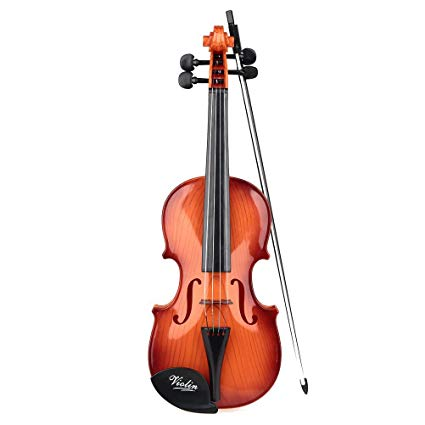
\includegraphics[width=.1\textwidth]{images/violin.jpg}};
        \draw[->] (-0.8, 0.5) -- (-0.2, 0.5);
        \draw[fill=cGreen!20] (0,0) -- (0,1) -- (1, 0.75) -- (1, 0.25) -- (0,0);
        \draw (0.5, 0.5) node{$f$};
        \draw[->] (1.2, 0.5) -- (1.8, 0.5);
        \draw (2, 0.5) node{$z$};
        \draw[->] (2.2, 0.5) -- (2.8, 0.5);
        \draw[fill=cGreen!20] (3,0.25) -- (3,0.75) -- (4, 1) -- (4, 0) -- (3,0.25);
        \draw (3.5, 0.5) node{$g$};
        \draw[->] (4.2, 0.5) -- (4.8, 0.5);
        \draw (5.5,0.5) node{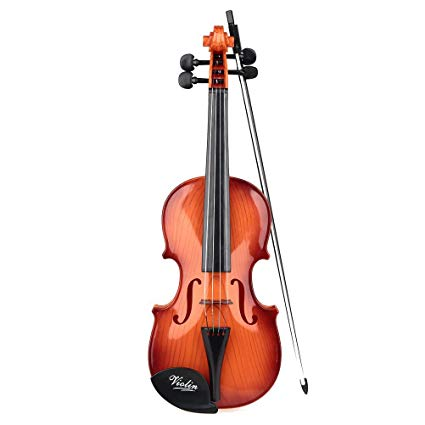
\includegraphics[width=.1\textwidth]{images/violin.jpg}};
        \end{tikzpicture}
    \end{figure}
    \begin{itemize}
        \item The goal is to learn an encoder $f$ and a decoder $g$ such that $g \circ f$ is close to identity.
        \item If $f$ and $g$ are linear, the optimal solution is given by a PCA
        \item Otherwise, we can achieve better performance with deep networks
    \end{itemize}
\end{frame}

\begin{frame}{Deep Autoencoders}
    \begin{figure}
        \centering
        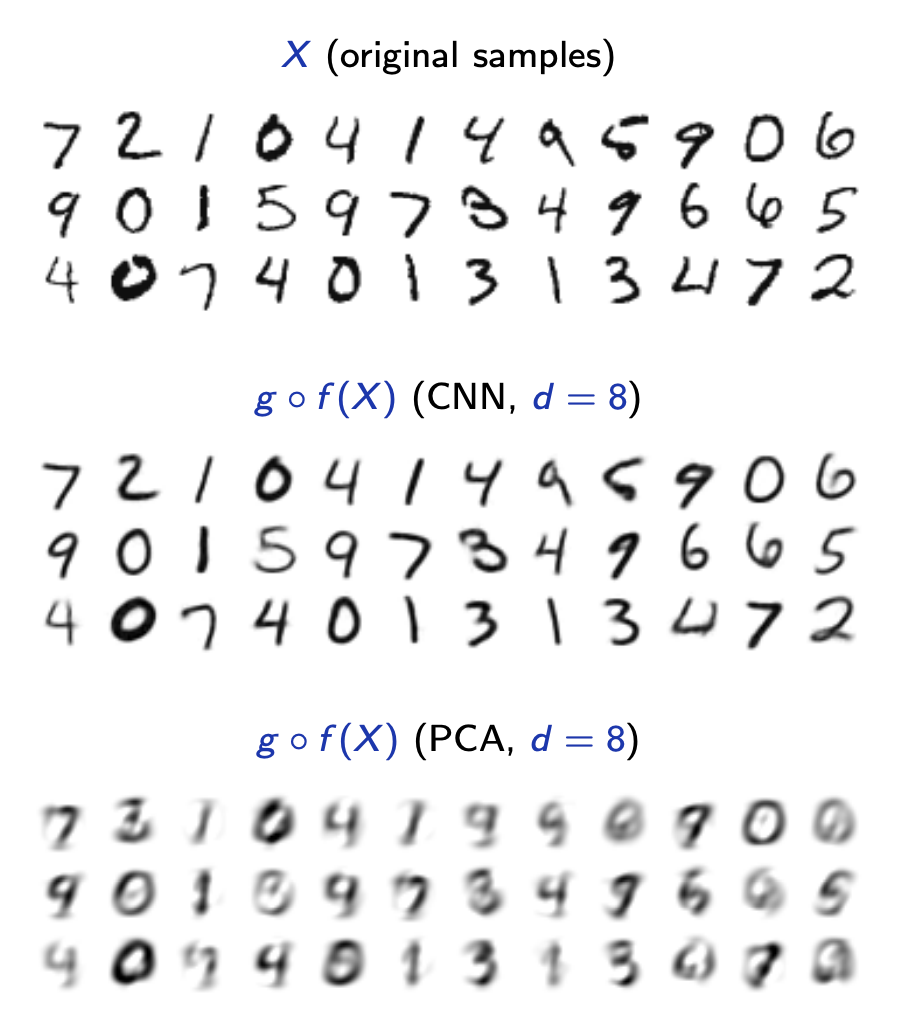
\includegraphics[width=0.6\linewidth]{images/ae_cnn_vs_pca.png}
        \caption*{(by courtesy of François Fleuret)}
    \end{figure}
\end{frame}

\begin{frame}{How to sample from autoencoders ?}

\begin{itemize}
    \item Simple answer: sample $z$ in the latent space and feed it into the decoder
    \item However it is very likely that the encoded inputs lies in a low-dimensional manifold inside the latent space
\end{itemize}
\begin{figure}
    \centering
    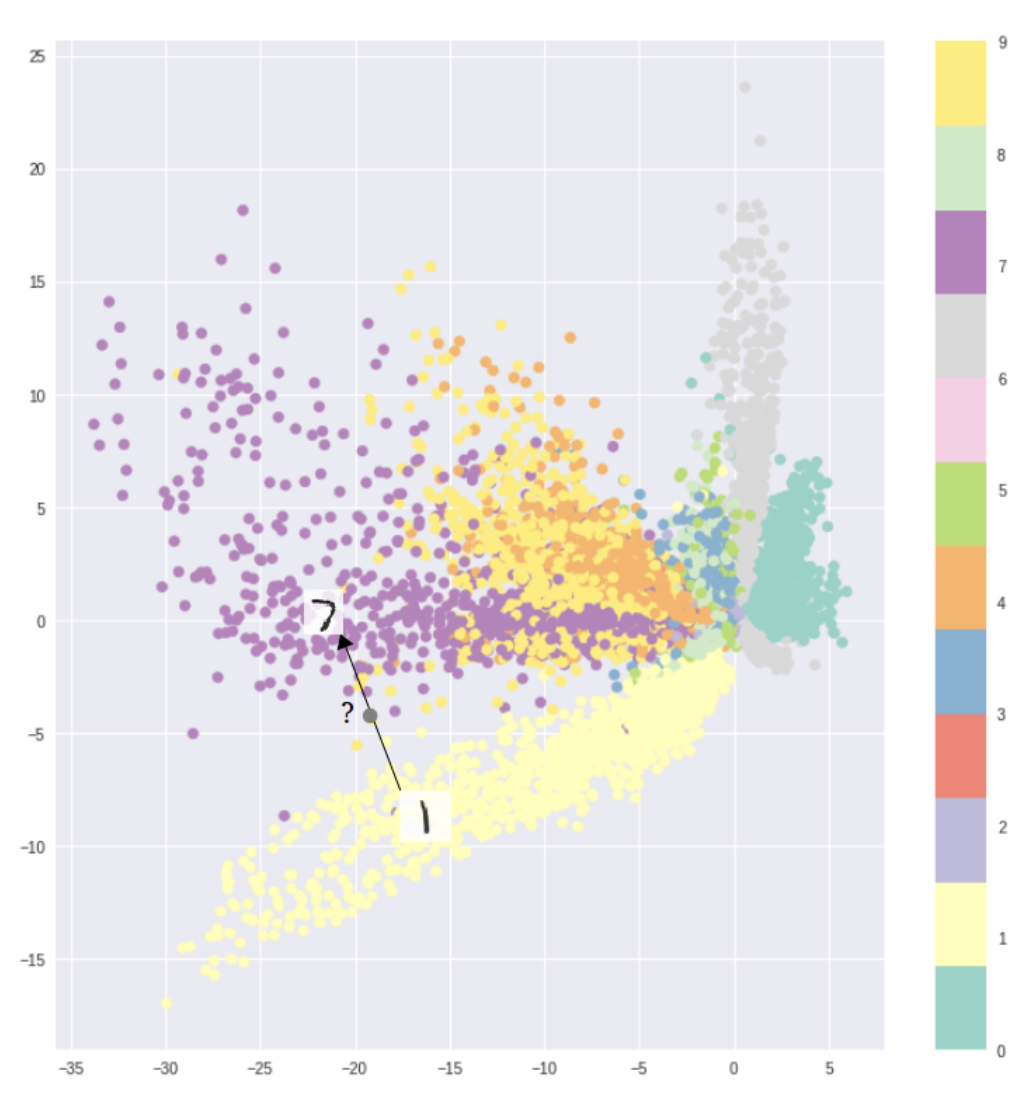
\includegraphics[width=0.5\linewidth]{images/latent_ae.png}
    \caption{Caption}
    \label{fig:my_label}
\end{figure}
\end{frame}

\begin{frame}{VAE in a nutshell}
    \begin{itemize}
        \item \textcolor{cGreen!80}{\textbf{Let us constraint the latent variable $z$ to follow a fixed distribution from which we can sample easily}}
        \item Let's rewrite everything with probabilities !
        \begin{figure}
        \centering
        \begin{tikzpicture}
        \draw (-1, 0.5) node{$x$};
        \draw[->] (-0.8, 0.5) -- (-0.2, 0.5);
        \draw[fill=cGreen!20] (0,0) -- (0,1) -- (1.5, 0.75) -- (1.5, 0.25) -- (0,0);
        \draw (0.75, 0.5) node{$p_\theta(z|x)$};
        \draw[->] (1.5, 0.5) -- (2.3, 0.5);
        \draw (2.5, 0.5) node{$z$};
        \draw[->] (2.7, 0.5) -- (3.3, 0.5);
        \draw[fill=cGreen!20] (3.5,0.25) -- (3.5,0.75) -- (5, 1) -- (5, 0) -- (3.5,0.25);
        \draw (4.25, 0.5) node{$p_\theta(x|z)$};
        \draw[->] (5, 0.5) -- (5.7, 0.5);
        \draw (6,0.5) node{$x'$};
        \end{tikzpicture}
    \end{figure}
    \item $p_\theta(z|x)$ is untractable since we do not know the distribution of the true data so we approximate it by the \textcolor{cOrange}{variational distribution $q_\phi(z|x)$} that should minimize
    \[ \mathbb{D}_{KL}(q_\phi(z|x), p_\theta(z|x)) \;\;. \] 
    %= \mathbb{E}_{z\sim q_\theta(z|x)} \left[ \mathop{log}(q_\phi(z|x)) - \mathop(log)(p_\theta(z|x)) \right]
    
    \end{itemize}
    
\end{frame}

\begin{frame}{VAE in a nutshell (cted)}
    \begin{lemma}
    For any variational distribution $q_\phi$, the (true) marginal log-likelihood $log(p_\theta(x))$ can be written as
        \[ \mathbb{D}_{KL}(q_\phi(z|x), p_\theta(z|x)) + \mathcal{L}_{\theta, \phi}\;\;. \]
    \end{lemma}

Note that:
    \begin{itemize}
        \item $\mathcal{L}_{\theta, \phi}$ is called the \textbf{variational lower bound} since $log(p_\theta(x)) > \mathcal{L}_{\theta, \phi}$
        \item For a fixed $\theta$, minimizing the KL-divergence wrt $\phi$ is similar to \textbf{maximize $\mathcal{L}_{\theta, \phi}$}.
        \item For a fixed $\phi$, maximizing $\mathcal{L}_{\theta, \phi}$ wrt $\theta$, maximizes the marginal log-likelihood of the data.
    \end{itemize}
\end{frame}

\begin{frame}{VAE in a nutshell}
\begin{itemize}
    \item Let's summarize ! The loss function to minimize is $-\mathcal{L}_{\theta, \phi}$ and can be rewritten as
    \[ \mathbb{E}_{z \sim q_\phi(z|x)} \left[ -log(p_\theta(x|z))\right] + \mathbb{D}_{KL}(q_\phi(z|x)|p_\theta(z)) \;\;. \]
    \item The first term is called the \emph{reconstruction loss}.
    \item The second term can be seen as a \emph{regularizer} toward the prior distribution of the latent variable $p_\theta$
\end{itemize}
\end{frame}

\begin{frame}{One last problem ! How to backprop ?}

\begin{itemize}
    \item \textbf{Problem:} Impossible to backpropagate through a \textbf{\textcolor{cBlue}{stochastic node}} like $z$\\
\end{itemize}
\begin{figure}
    \centering
    \begin{tikzpicture}
        \draw (-1, 0.5) node{$x$};
        \draw[->] (-0.8, 0.5) -- (-0.2, 0.5);
        \draw[fill=cGreen!20] (0,0) -- (0,1) -- (1, 0.75) -- (1, 0.25) -- (0,0);
        \draw (0.5, 0.5) node{$f$};
        
        \draw[->] (1.2, 0.5) -- (1.7, 0);
        \draw[->] (1.2, 0.5) -- (1.7, 1);
        \draw (2, 1) node{$\mu_z$};
        \draw (2, 0) node{$\sigma_z$};
        
        \draw[->] (2.3, 0) -- (2.6, 0.3);
        \draw[->] (2.3, 1) -- (2.6, 0.7);
        
        \draw (3, 0.5) node[circle,radius=0.5cm,fill=cBlue!50]{$z$};
        
        \draw[->] (3.5, 0.5) -- (4.1, 0.5);
        \draw[fill=cGreen!20] (4.3,0.25) -- (4.3,0.75) -- (5.3, 1) -- (5.3, 0) -- (4.3, 0.25);
        \draw (4.8, 0.5) node{$g$};
        \draw[->] (5.5, 0.5) -- (6.1, 0.5);
        \draw (6.3, 0.5) node{$x$};
    \end{tikzpicture}
\end{figure}
\begin{itemize}
    \item \textbf{Solution:} Let's write $z = \mu_z + \sigma_z \odot \epsilon$ with $\epsilon \sim \mathcal{N}(0,1)$ to have a differentiable path end-to-end.
\end{itemize}
\begin{figure}
    \centering
    \begin{tikzpicture}
        \draw (-1, 0.5) node{$x$};
        \draw[->] (-0.8, 0.5) -- (-0.2, 0.5);
        \draw[fill=cGreen!20] (0,0) -- (0,1) -- (1, 0.75) -- (1, 0.25) -- (0,0);
        \draw (0.5, 0.5) node{$f$};
        
        \draw[->] (1.2, 0.5) -- (1.7, 0);
        \draw[->] (1.2, 0.5) -- (1.7, 1);
        \draw (2, 1) node{$\mu_z$};
        \draw (2, 0) node{$\sigma_z$};
        
        \draw[->] (2.3, 0) -- (2.6, 0.3);
        \draw[->] (2.3, 1) -- (2.6, 0.7);
        
        \draw (3, 0.5) node{$z$};
        
        \draw (3, -0.5) node[circle,radius=0.5cm,fill=cBlue!50]{$\epsilon$};
        \draw[->] (3, -0.1) -- (3, 0.2);
        
        \draw[->] (3.5, 0.5) -- (4.1, 0.5);
        \draw[fill=cGreen!20] (4.3,0.25) -- (4.3,0.75) -- (5.3, 1) -- (5.3, 0) -- (4.3, 0.25);
        \draw (4.8, 0.5) node{$g$};
        \draw[->] (5.5, 0.5) -- (6.1, 0.5);
        \draw (6.3, 0.5) node{$x$};
    \end{tikzpicture}
\end{figure}
\begin{center}
    \textbf{\textcolor{cOrange}{Reparametrization trick}}
\end{center}
\end{frame}

\section{Generative Adversarial Nets}

\begin{frame}{GANs}
\textbf{New idea by \cite{gan}: let us write the problem as a minimax game between a \emph{generator} and a \emph{discriminator}}
    \begin{figure}
        \centering
        \begin{tikzpicture}[scale=0.7,every node/.style={scale=0.7}]
        \draw (-3,0.75) node{random seed};
        \draw[bigarrow] (-1.5, 0.75) -- (-0.75, 0.75);
        \draw[fill=cBlue!20] (-0.5,0.4) -- (-0.5,1.1) -- (2.5, 1.8) -- (2.5, -0.3) -- (-0.5,0.4);
        \draw (1, 0.75) node{Generator};
        \draw[bigarrow] (2.5, 0.75) -- (3.5, 0.75) -- (3.5, -1);
        
        \draw (2,-2.8) node{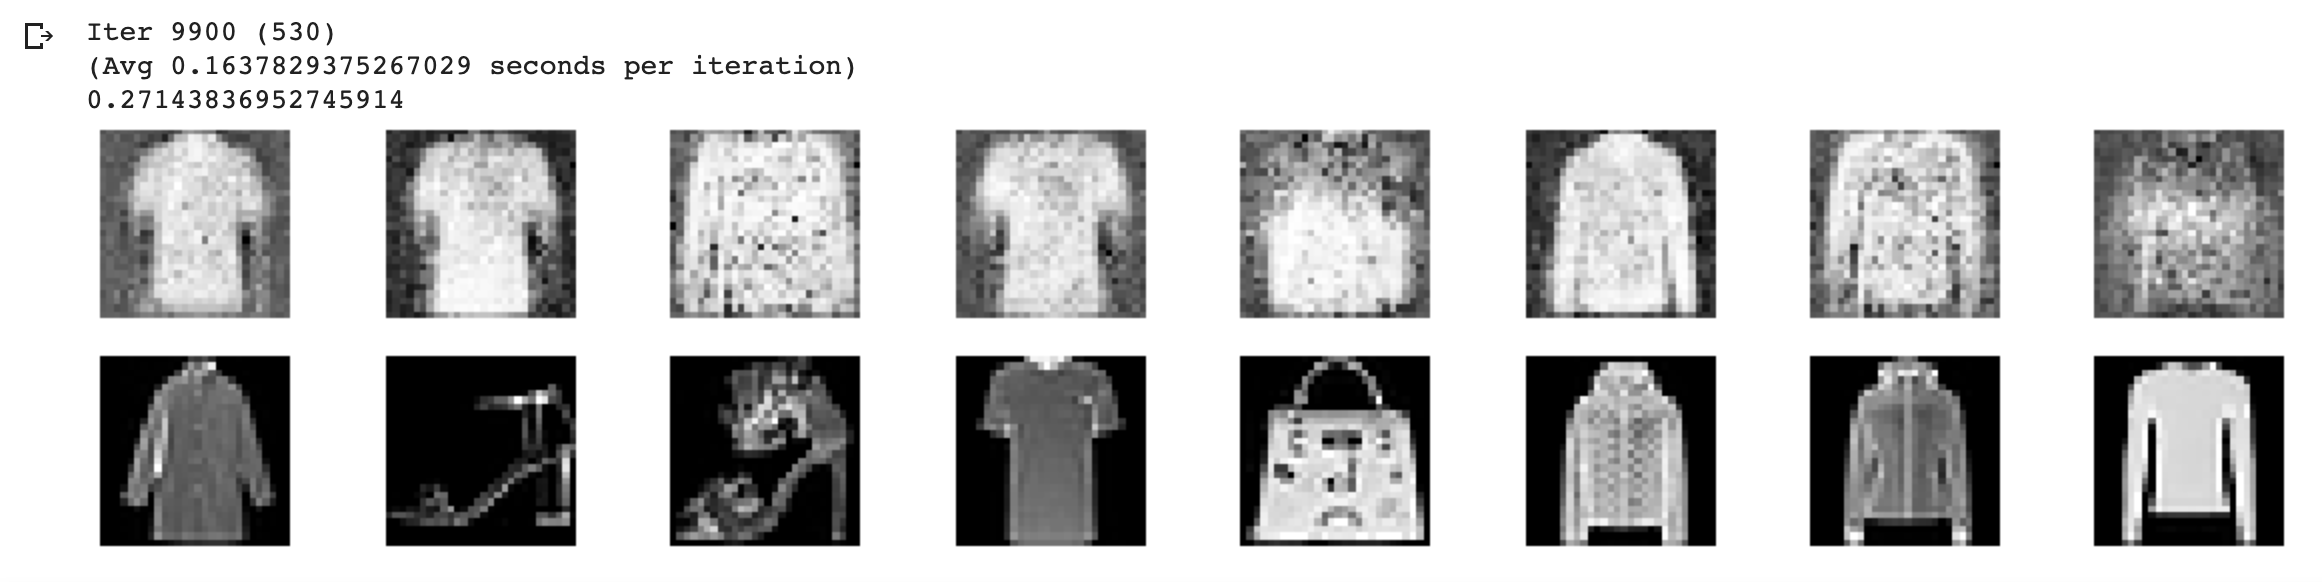
\includegraphics[width=1.2\textwidth]{images/fashion_gan.png}};
        
        \draw (-3,-6) node{real images};
        \draw[bigarrow] (0, -6) -- (3.5, -6) -- (3.5, -5);
        
        \draw[bigarrow] (8.5,-3) -- (9,-3);
        \draw[fill=cOrange!20] (9,-4) -- (9,-2) -- (12, -2.5) -- (12, -3.5) -- (9,-4);
        \draw (10.4, -3) node{Discriminator};
        \end{tikzpicture}
    \end{figure}
\end{frame}

\begin{frame}{GANs (cted)}
    \begin{itemize}
        \item Let us consider a generator $G$ parametrized by $\theta$ and a discriminator $D$ parametrized by $\phi$\\
        and
            \begin{itemize}
                \item $(x^i)_{i=1\dots n}$ a batch of $n$ training images
                \item $(z^i)_{i=1\dots n}$ a batch of $n$ noise samples sampled from a fixed noise prior.
            \end{itemize}
        \item The goal of the discriminator is to distinguish between $G(z)$ and $x$ so \textcolor{cOrange}{minimize} the negative log-likelihood
        \textcolor{cOrange}{\[ NLLH(x,z, \theta) = -\left[ \sum_{i=1}^n log(D_\theta(x^i)) + log(1-D_\theta(G_\phi(z^i)) \right] \;\;. \]}
        \item The goal of the generator is to \textcolor{cBlue}{minimize} the log-likelihood
        \textcolor{cBlue}{\[ LLH(x,\phi) = \sum_{i=1}^n log(1-D_\theta(G_\phi(z^i)) \]}
    \end{itemize}
\end{frame}

\begin{frame}{GANs :: Pathological behaviors}
\begin{itemize}
    \item \textbf{Oscillation / bad convergence}~\\
    Due to minimax game
    \item \textbf{Mode collapse}~\\
    Happens when the training data is multi-modal (which is usually the case in practice): can be a good strategy for the generator to target the easiest mode of the target distribution (pullover in the example below)
\end{itemize}
\end{frame}

\begin{frame}{GANs :: Alchemy ?}
Lots of "hacks" to stabilize the training
    \begin{enumerate}
        \item Normalize the inputs
        \item $\mathop{min} log(1-D)$ vs $\mathop{max} log(D)$
        \item Choose the noise prior wisely
        \item BatchNorm on full real / fake images
        \item Avoid Sparse Gradients (ReLu -> LeakyReLu)
        \item Use soft / noisy labels
        \item Choose the optimizers wisely (e.g. Adam for G, SGD for D)
        \item \dots
    \end{enumerate}
    (from https://github.com/soumith/ganhacks)
\end{frame}

\begin{frame}{GANs :: (A bit of) theory}
    \begin{itemize}
        \item Let us denote 
            \begin{itemize}
                \item $\mu$ the density of the true data
                \item $\mu_G = G(\mu_\text{noise})$ the density of the data generated by a generator $G$
            \end{itemize}
        \item Our main goal is to find $G$ that minimizes the distance between $\mu$ and $\mu_G$
        \item \textcolor{cOrange}{\textbf{Intuition}}: the bigger gap between $\mu$ and $\mu_G$, the better the optimal discriminator.
    \end{itemize}
    
    \begin{center}
        \textcolor{cBlue}{\textbf{Can we formalize this intuition ?}}
    \end{center}
    
    
    
\end{frame}

\begin{frame}{GANs :: (A bit of) Theory}
    \begin{theorem}
        The optimal discriminator (without regularization) $D^\ast_G$ is
        \[ \textcolor{cRed}{x \to \frac{\mu(x)}{\mu(x)+\mu_G(x)}} \;\;. \] 
        The corresponding loss at this point is 
        \[ \textcolor{cRed}{\mathcal{L}_G(D^\ast_G) = 2 \mathbb{D}_{JS}(\mu, \mu_G) - \mathop{log}(4)} \;\;, \]
        where $\mathbb{D}_{JS}$ is the Jensen-Shannon divergence (symmetric variant of the KL-divergence).
    \end{theorem}
    
    \begin{center}
        \textcolor{cBlue}{\textbf{Training the GAN $\equiv$ finding $G$ that minimizes $\mathbb{D}_{JS}(\mu, \mu_G)$}}
    \end{center}
\end{frame}


\begin{frame}{Wasserstein GANs}
\begin{itemize}
    \item \cite{wgan} claims that the Jensen-Shannon divergence does not allow to take into account the metric structure of the space.
    \item They proposes to go with the Wasserstein distance $\textcolor{cBlue}{\mathbb{D}_{W_1}}$.
    \[ \textcolor{cBlue}{\mathbb{D}_{W_1}(\mu, \nu) = \mathop{inf}_{\gamma \in \Gamma(\mu, \nu)} \int d(x,y) d\gamma(x,y)} \]
    \item "earth moving distance"
\end{itemize}
\begin{figure}
    \centering
    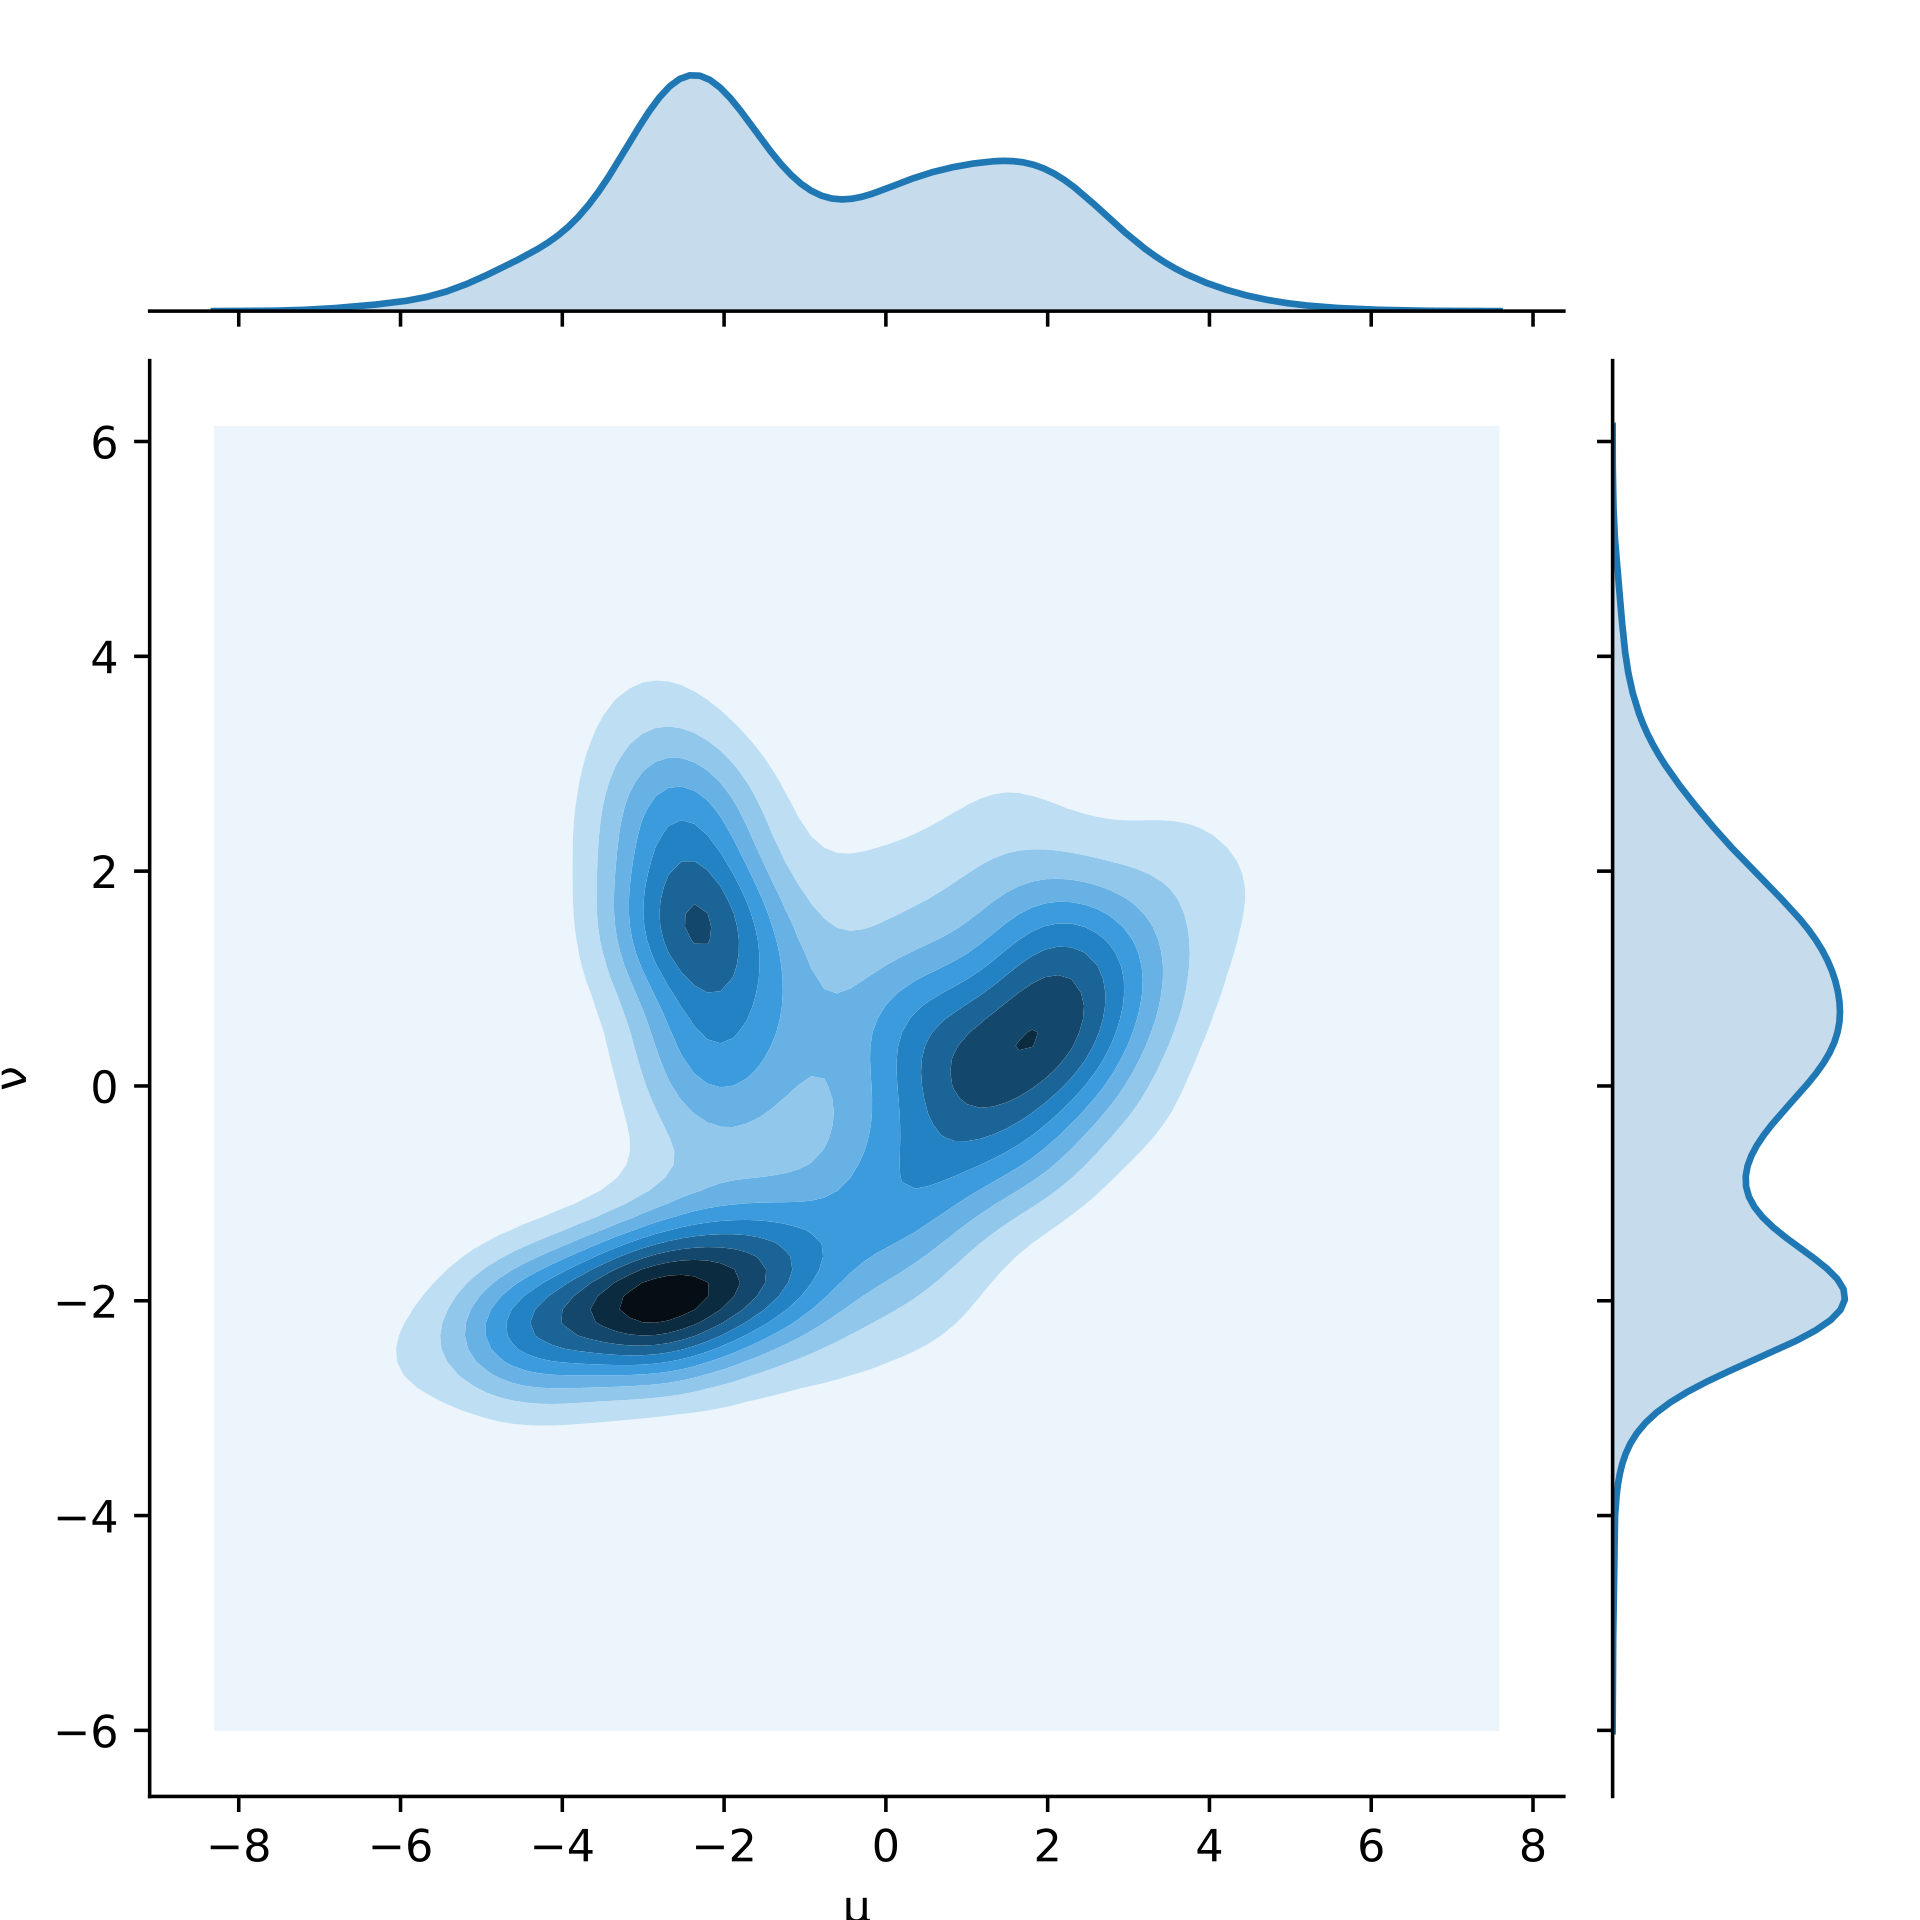
\includegraphics[width=0.35\linewidth]{images/wasserstein.png}
\end{figure}
\end{frame}

\begin{frame}{Wasserstein GANs (cted)}
Advantages of $\mathbb{D}_{W_1}$ over $ \mathbb{D}_{JS}$ ?

\begin{figure}
    \centering
    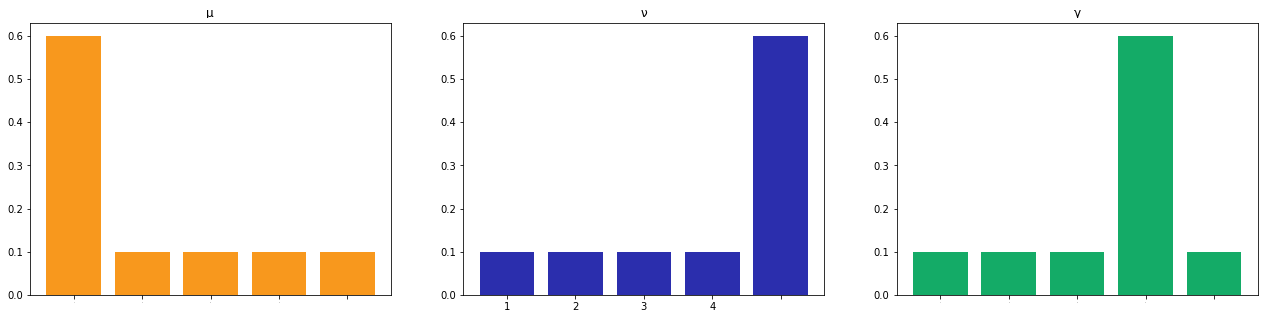
\includegraphics[width=0.95\linewidth]{images/distrib.png}
\end{figure}

\[ \mathbb{D}_{W_1}(\textcolor{cOrange}{\mu}, \textcolor{cBlue}{\nu}) = 2 > \mathbb{D}_{W_1}(\textcolor{cOrange}{\mu}, \textcolor{cGreen}{\gamma}) = 1.5 \]

\[ \mathbb{D}_{JS}(\textcolor{cOrange}{\mu}, \textcolor{cBlue}{\nu}) = 0.20 < \mathbb{D}_{JS}(\textcolor{cOrange}{\mu}, \textcolor{cGreen}{\gamma}) = 0.25 \]

\begin{center}
    \textcolor{cRed}{\textbf{Problem}: How to compute $\mathop{argmin}_G \mathbb{D}_{W_1}(\mu, \mu_G)$ ?}
\end{center}
\end{frame}

\begin{frame}{Wasserstein GANs (cted)}
    \begin{itemize}
        \item Using \textcolor{cOrange}{Kantorovich-Rubinstein duality theorem},
        \[ \mathbb{D}_{W_1}(\mu, \mu_G) = \mathop{max}_{\Vert D \vert_L \leq 1} \left[ \mathbb{E}_{X\sim \mu}\left[ D(X) \right] - \mathbb{E}_{X\sim \mu_G}\left[ D(X) \right] \right] \;\;, \]
        where $\Vert D \vert_L$ is the \textcolor{cOrange}{Lipschitz semi-norm} equal to
        \[ \mathop{max}_{x,y} \frac{\Vert D(x)-D(y) \Vert }{\Vert x-y \vert} \;\;. \]
        \item We get a \textcolor{cBlue}{\textbf{new loss}} for the discriminator !
        \item Main issue is to deal with the semi-norm constraint !
        \begin{itemize}
            \item Weight clipping (original idea)
            \item Smooth penalty (\cite{iwgan})
        \end{itemize} 
    \end{itemize}
\end{frame}

\begin{frame}{Conditional GANs}
    
\end{frame}

\begin{frame}{Cycle GANs}
    
\end{frame}

\begin{frame}{Image 2 Image}
    
\end{frame}


\section{Wrapping up}

\begin{frame}{VAE vs GANs}
    \begin{figure}
        \centering
        \begin{tabular}{|c|c|c|}
                \hline
                \cellcolor{cBlue!20} & \cellcolor{cBlue!20} VAE & \cellcolor{cBlue!20} GAN \\
                \hline
                \hline
                Modules & Encoder + Decoder & Generator + Discriminator \\
                \hline
                Training ? & Reconstruction Loss & Minimax game \\
                & + Latent Loss & \\
                \hline
                Stability ? & \cellcolor{cGreen!50} Closed-form & \cellcolor{cRed!50} Need to reach \\
                & \cellcolor{cGreen!50} & \cellcolor{cRed!50} a \emph{Nash} equilibrium  \\
                \hline
                Quality ? & \cellcolor{cOrange!50} Good but  & \cellcolor{cGreen!50} High quality \\
                & \cellcolor{cOrange!50} blurry images & \cellcolor{cGreen!50} sharp images \\
                \hline
                \hline
        \end{tabular}
    \end{figure}
\end{frame}



\section*{References}

\begin{frame}[allowframebreaks]\small
  \frametitle{References}
  \renewcommand*{\bibfont}{\footnotesize}
  \printbibliography
\end{frame}

\end{document}
